% Preamble {{{
\documentclass[11pt,a4paper,titlepage,dvipsnames,cmyk]{scrartcl}
\usepackage[english]{babel}
\typearea{12}
% }}}

% Set indentation and line skip for paragraph {{{
\setlength{\parindent}{0em}
\setlength{\parskip}{1em}
\usepackage[margin=2cm]{geometry}
\addtolength{\textheight}{-1in}
\setlength{\headsep}{.5in}
% }}}

\usepackage{hhline}
\usepackage[table]{xcolor}
\usepackage{mathtools}
\usepackage{tabularx}
\usepackage[T1]{fontenc}

% Headers setup {{{
\usepackage{fancyhdr}
\pagestyle{fancy}
\lhead{Cloud Computing and Big Data}
\rhead{Josh Felmeden}
\usepackage{hyperref}
% }}}

% Listings {{{
\usepackage[]{listings}
\lstset
{
    breaklines=true,
    tabsize=3,
    showstringspaces=false
}

\definecolor{lstgrey}{rgb}{0.05,0.05,0.05}
\usepackage{listings}
\makeatletter
\lstset{language=[Visual]Basic,
backgroundcolor=\color{lstgrey},
frame=single,
xleftmargin=0.7cm,
frame=tlbr, framesep=0.2cm, framerule=0pt,
basicstyle=\lst@ifdisplaystyle\color{white}\footnotesize\ttfamily\else\color{black}\footnotesize\ttfamily\fi,
captionpos=b,
tabsize=2,
keywordstyle=\color{Magenta}\bfseries,
identifierstyle=\color{Cyan},
stringstyle=\color{Yellow},
commentstyle=\color{Gray}\itshape
}
\makeatother
\renewcommand{\familydefault}{\sfdefault}
\newcommand{\specialcell}[2][c]{%
\begin{tabular}[#1]{@{}c@{}}#2\end{tabular}}
% }}}

% Other packages {{{
\usepackage{graphicx}
\graphicspath{ {./pics/} }
\usepackage{needspace}
\usepackage{tcolorbox}
\usepackage{soul}
\usepackage{babel,dejavu,helvet}
\usepackage{amsmath}
\usepackage{booktabs}
\usepackage{tcolorbox}
\usepackage[symbol]{footmisc}
\renewcommand{\thefootnote}{\fnsymbol{footnote}}
\renewcommand{\familydefault}{\sfdefault}
\usepackage{enumitem}
\setlist{nolistsep}
% }}}

% tcolorbox {{{
\newtcolorbox{blue}[3][] {
colframe = #2!25,
colback = #2!10,
#1,
}

\newtcolorbox{titlebox}[3][] {
colframe = #2!25,
colback = #2!10,
coltitle = #2!20!black,
title = {#3},
fonttitle=\bfseries
#1,
}
% }}}

% Title {{{
\title{Cloud Computing and Big Data}
\author{Josh Felmeden}
% }}}

\begin{document}
\maketitle
\tableofcontents
\newpage
\section{Overview}
\subsection{Economic Driving Factors}
Cloud computing works by charging someone to use a service for a certain amount of time. If, for example, you let someone use your computer, you might charge them for their usage (if you were a real meanie). How that would be worked out is the \textit{operation expenditure} (Opex) and the \textit{capital expenditure} (Capex, cost of the computer). Combining these, we calculate the \textit{total cost of operation} and calculate the cost per day of the lifespan of the computer (in this example). So, if you used the computer for an hour, you would owe the person a 24th of this daily cost.

Now, this might come down to half a penny, but of course, this doesn't exist any more, so we might charge a whole penny instead. This seems like a marginal profit, but in terms of percentages, this is a $100\%$ increase. The fundamentals of this are how cloud computing generates so much income.

The attraction of this is that the users of the services do not have to pay the Capex, and simply pay opex for the rental of the service.

\subsection{Normal Failure}
Failures in these systems are to be expected. Say the servers you are buying are guaranteed to have a $99.999\%$ 3-year survival rate (`five-nines reliability'). This is good because there is a very high chance that this remains. Now, if you buy 10 of these servers, the probability that you have all of the servers still working is only $99.99\%$. Taking this to the extremes, if you buy 500,000 servers (this is standard practise for a lot of the big servers these days), the probability that all of them are still working is a measly $1\%$. Essentially, failure is something that should be normalised.

\textit{Modular data centres} are used a lot in big data centres. A unit may be left in the shipping container, and this container is removed or added as a container, meaning that if one module fails, another can just be replaced, meaning that the whole centre doesn't collapse.

In the current climate, the modular centres are considered a whole working unit, and this way of thinking was mobilised by a group of Google engineers.

\subsection{Blank as a service (XaaS)}
\begin{itemize}
    \item \textbf{SaaS: Software as a service}
    \begin{itemize}
        \item End user application software that is remotely delivered over the internet.
        \item Adobe is an example of this (Adobe Creative Cloud)
        \item Used to be bought off the shelf as a CD
    \end{itemize}
    \item \textbf{PaaS: Platform as a Service}
    \begin{itemize}
        \item Developer application software (middleware) functionality is remotely accessible
        \item Might provide a particular combination of OS, web-server, data-base and scripting
        \item Popular instance is the free `LAMP stack' (Linux, Apache, MYSQL and PHP)
        \item Used to be dominated by \textit{Google}
    \end{itemize}
    \item \textbf{IaaS: Infrastructure as a Service}
    \begin{itemize}
        \item IT infrastructure almost always virtualised and remotely accessible.
        \item Virtualisation software allows one physical server to be used by multiple users, each on a virtual machine. If one crashes, the others keep running.
        \item Used to be dominated by \textit{AWS} (although this is now a much bigger thing).
    \end{itemize}
\end{itemize}

While Google and Amazon dominated their respective fields, both of these companies have expanded into the other fields. This is very complicated, but the key thing is that both Google and Amazon offer both PaaS and IaaS.

In around 2015, Amazon created \textbf{FaaS: function as a service (aka `serverless')}:
\begin{itemize}
    \item No server processes visibly running. Pay only for the time spent executing a function
    \item UNlike PaaS, scale out without increasing number of servers.
    \item Amazon Lambda is the best known example, although both Google and Microsoft have answers to this.
\end{itemize}

\subsection{Impacts of Cloud Services}
Cloud services have revolutionised business in many ways. It is now possible to do tasks that would previously require access to high performance machines. Instead, it can be sent to a big data centre, and this usage is just charged as rental.

\textit{Interoperability} is a big issue. \textbf{Vendor lock-in} is a concern for a lot of clients, and this simply means that once a client is locked into a vendor, it becomes financially or practically unviable to switch to another supplier. This led to an attempt to develop a sense of unity between cloud companies, where companies created the \textit{Open Cloud Manifesto}. A lot of big companies signed up to this, but a lot of the top dogs didn't sign up for this (unsurprisingly, Google and Amazon). This manifesto seemingly no longer exists as an original. As a consumer, this is bad and worrying because vendor lock in is very possible.

\section{IaaS and AWS}
\subsection{Amazon Simple Storage Service (S3)}
Amazon S3 is a cloud-based persistent storage. It operates independently from other Amazon services. The `simple' refers to the features, not that it's simple to use. You can store data in the cloud. You also don't store files, you store \textit{objects}, and these are kept in buckets. Objects have a size limit (5Tb) and a max size on a single upload is 5Gb. All buckets share the same namespace, so no sub-buckets.

It's very easy to use; just use a web GUI that is similar to AWS. It also has a command line interface and has scripting. Default storage can be selected (geographically).

S3 is accessed via API, either by SOAP (xml) or REST (http). Wrappers are available to abstract the API for programmers.

This is just the storage, so now we will look at the computing of data in the cloud.

\subsection{Amazon Elastic Compute Cloud (EC2)}
This is a remotely accessible virtual network of virtual servers. Usually, EC2 is run with S3 providing the storage.

A single EC2 virtual server, with the chosen OS etc, is an instance. An instance is instantiatied from an Amazon Machine Image (AMI)
\begin{itemize}
    \item One AMI can be cloned $n$ times to create $n$ instances
    \item You can build your own by cloning an AMI from your local server
    \item Or, Amazon have a bunch of prebuilt AMIs that you can choose from
\end{itemize}

EC2 dynamically assigns a unique IP address to each instance, and this IP can be reassigned, perhaps to someone else. The IP can also be static (also known as an Elastic IP address) at a cost.

EC2 instances run in availability zones (AZs), grouped into regions. AZ is similar to a single data centre, guaranteeing an area has 99.95\% uptime.

\subsubsection{Usage}
Some basic API routes as S3, command-line or a bit of GUI too:
\begin{itemize}
    \item Amazon's own AWS web console
    \item Various EC2 plug-ins for browsers
    \item Third-party cloud management tools
\end{itemize}

Some AMIs are junk or malware, however, so be careful when selecting this.

There are three types of storage:
\begin{itemize}
    \item Ephemeral local storage in the instance (dies with instance)
    \item Persistent cloud (S3)
    \item SAN-style Elastic Block Storage (EBS)
    \begin{itemize}
        \item Allows user to create volumes from 1Gb to 1Tb
        \item Any number of volumes may be mounted from a single instance
    \end{itemize}
\end{itemize}

S3 is slow, medium-reliable, but super-durable. Never loses data, so is good for DR backups. Instance storage is simple and cheap, but speed can be really poor. EBS is high on everything, but is complex and costly.

There is some autoscaling based on metrics:
\begin{itemize}
   \item \textbf{Cloudwatch}: automated monitoring of EC2 instances. Reveals many statistics such as CPU utilisation, disk reads/writes and network traffic. Aggregates and stores monitoring data that can be accessed
   \item \textbf{Auto Scaling}: dynamically adds or removes EC2 instances based on CloudWatch metrics. You define conditions upon which you want to scale up or down your EC2 instances. Auto scaling automatically adds or removes the specified amount of Amazon EC2 instances when it detects that the conditions have been met.
   \item \textbf{Elastic Load Balancing}: automatically distributes incoming application traffic across multiple EC2 instances. Better fault tolerance. Elastic Load Balancing detects unhealthy instances within a pool and automatically reroutes traffic to healthy instances until the unhealthy instances have been restored. Customers can enable ELB within a single AZ or across multiple for consistent application performance.
\end{itemize}

\subsection{AWS Simple Queue Service (SQS) and Architecting for Scale-out}
SQS is reliable, loosely-coupled fault-tolerant storage and delivery of messages. It can be between any clients or computers connected to the internet, and senders and recipients do not have to communicate directly. No requirement that either side be always-available or connected to the internet.

A \textbf{message} is up to 256Kb of text-data, sent to SQS and stored until it is delivered. A \textbf{queue} serves to group related messages together.

SQS is accessible to clients on any HTTP-enabled platform. Messages are stored redundantly over multiple data-centres truly distributed. Unfortunately, this brings about a few down-sides:
\begin{itemize}
    \item Message retrievals may be incomplete
    \item Messages may not be delivered quickly (2-10 seconds)
    \item Messages may be delivered out of order
    \item Messages may be redelivered
\end{itemize}

\subsubsection{Mitch Garnaat's Monster Muck Mashup}
This is a service that converts AVI videos to mp4 using:
\begin{itemize}
    \item `Boto' Python interface to AWS
    \item S3 to store the video files
    \item EC2 to do the conversion processing
    \item SQS for inter-process communication
\end{itemize}

Uses AWS for \textit{scalability} (scale-out not up, not just buying new resources, adding cheap machines to improve ability.)

The basic steps are:
\begin{enumerate}
\item Upload a bunch of video files to a S3 bucket
\item For each file, add a msg to SQS input queue
\item On the EC2 instance, repeat this until input queue is empty:
\begin{enumerate}
    \item Read message MI from input queue
    \item Retrieve from S3 the video VI specified in MI
    \item Do the conversion creating VO
    \item Store VO in S3
    \item Write message MO to SQS output queue
    \item Delete MI from input queue
\end{enumerate}
\end{enumerate}

This really illustrates how good AWS is at scaling software. It is good because any number of clients can connect to the bucket. If this bucket is 100\% full, it doesn't matter, because additional instances can all talk to the same buckets and queues, so the workload is met.

\subsection{AWS simpleDB and AWS Relational Databases (RDB)}
\subsubsection{Amazon SimpleDB}
This software provides:
\begin{itemize}
    \item Reliable storage of structured textual data
    \item Languages that allows you to store, modify, query, and retrieve data sets
    \item Automatic indexing of all stored data
\end{itemize}

SimpleDB provides 3 main resources:
\begin{itemize}
    \item \textbf{Domains}: Highest-level container for related data \textit{items}: queries only search within one domain
    \item \textbf{Items}: a named collection of \textit{attributes} that represent a data object. Each item has a unique name within the domain; items can be created, modified, or deleted; individual attributes within an an item can be manipulated
    \item \textbf{Attributes}: an individual category of information within the item, with a name unique for that item. Item has one or more text string values associated with the name
\end{itemize}

The downside to this type of storage is that it really does only do one data type (textual). If, for example, you wanted to store pi, you would need to store it as a character string (`3', `.', `1').

There is no Database \textbf{schema}, meaning if you mistype something, the database will just accept it as a definition, leading to some unfortunate results. It is not a traditional relational database management system:
\begin{itemize}
    \item SimpleDB items are stored in a hierarchical structure, not a table
    \item SimpleDB attribute value max size is 1Kb
    \item SimpleDB data is all stored as text
    \item The query language is really basic
    \item SimpleDB is distributed, so data consistency may suffer due to propagation delays
\end{itemize}

\subsubsection{Amazon Relation Database Service}
There is also a relational database system, possibly as a response to Azure. You can set up, operate and scale a full MySQL RDBMS without having to worry about infrastructure provisioning, software maintenance, or common DB management tasks, like backups.

The processing power and storage space can be scaled as needed with a single API call and you can fully initiate fully consistent database snapshots at any time. Can import a dump file to get started. Each DB instance exports a number of metrics to CloudWatch including CPU utilisation, etc.

\subsection{Availability Zones}
Availability zones are clusters of independent data centres that are up to 20 miles apart. They are interconnected using low latency and enable fault isolation and HA.

Choosing which region to use comes down to a few reasons:
\begin{itemize}
    \item Data sovereignty and compliance
    \begin{itemize}
        \item Where are you storing user data?
    \end{itemize}
    \item Proximity of users to data
    \item Services and feature availability
    \item Cost effectiveness
    \begin{itemize}
        \item Each region has differing costs
    \end{itemize}
\end{itemize}

High Availability (HA) is the ability to minimise service downtime by using redundant components. It also requires service components in at least two AZs.

Fault tolerance is the same as HA, but also the ability to ensure that no service disruption by using active-active architecture meaning that all components are active all the time. This is of course a lot more costly that just having HA.

IaaS may have HA, but FT unlikely. PaaS will usually have HA, but some services offer FT.

\section{Virtualisation}
The most fundamental type of cloud computing is IaaS compute, and the most fundamental type of this is the virtual machine. It has unmanaged services, which means you control what they do. You create, save or reuse them. They are networked and connected to storage and have certain security systems.

EC2 instances are a form of virtualisation.
\begin{itemize}
    \item They mostly run on Xeon processors, but also have other processors available.
    \item There are lots of different tiers available on AWS that use different purposes
    \item They run in AMIs.
    \item After creating a virtual machine, you can start, stop, and terminate the machines. Once the machine is terminated, it will not come back.
\end{itemize}

In virtualisation, there is some virtual memory that points to addresses in physical memory. It is an abstraction of the storage resources, because the virtual memory seems contiguous, but in physical memory it could be in various locations. The operating system manages this and also has hardware support.

\begin{center}
    \begin{tabularx}{\textwidth}{X|X}
        \textbf{Virtual Memory} & \textbf{Virtual Machine} \\ \midrule
        Abstraction of the RAM memory resources & Abstraction of the storage/process/IO resources. \\
        Mapping of program (virtual) memory addresses to physical addresses & Time slicing VM use of virtual memory addresses/CPU/IO registers in physical addresses. \\
        Operating system manages & Operating system/Hypervisor manages \\
        Hardware support (memory management unit) & Hardware support (e.g. Intel VT)
    \end{tabularx}
\end{center}

\subsection{The hypervisor}


This virtualisation is not a new idea. It has been in use since around 1960, but it has been formalised in 1974, where they defined three important properties:
\begin{itemize}
    \item \textit{Fidelity}: Program gets the same output whether on VM or hardware
    \item \textit{Performance}: Performs close to physical computer
    \item \textit{Safety}: Cannot change or corrupt data on physical computer
\end{itemize}

This was ensured by analysing the instruction sets and identified two instructions that are the most important: \textbf{sensitive} instructions (that can change configurations of resources) and \textbf{privileged} instructions. Sensitive instructions need to be caught by the operating system, jumping from user mode to kernel mode. Therefore, all sensitive instructions need to be a subset of privileged instructions. This is all handled by the hypervisor.

Therefore, we have the hypervisor in contact with the server hardware, and then on top of this, we have the VM (or multiple machines) that consist of a guest OS, middleware, and apps. This type of VM is called \textbf{bare metal}.

Another type, called \textbf{hosted}, has a host OS running on top of the server hardware, and then the hypervisor.

The difference between the two is clear; in type two, the hypervisor can write to the host OS meaning that it can be more lightweight, where as type one can be much faster, at the cost of having to contain stuff that is normally handled by the OS.

\subsubsection{Simulated Hardware}
\textit{Full virtualisation} is a complete or almost complete simulation of the underlying guest-machine hardware: virtualised guest OS runs as if it were on a bare machine.

The alternative to this is \textit{paravirtualisation} and is only possible when the source code of the OS is available. The guest OS is edited and recompiled to make system calls into the hypervisor API to execute safe rewrites of sensitive instructions. In this example, the hypervisor doesn't simulate hardware.

EC2 offers both of these virtual machines:
\begin{itemize}
    \item HVM --- hardware virtual machine
    \begin{itemize}
        \item Virtualised set of hardware
        \item Can use OS without modification
        \item Intel virtualisation technology
    \end{itemize}
    \item PV --- Paravirtualisation
    \begin{itemize}
        \item Requires OS to be prepared
        \item Doesn't support GPU instances
    \end{itemize}
\end{itemize}

\subsubsection{Xen}
Xen is a free, open-source hypervisor developed at University of Cambridge. It has multiple modes:
\begin{itemize}
    \item Paravirtualisation: guest OS recompiled with modifications
    \item Hardware assisted virtualisation: Intel x86 and ARM extensions
    \item Widespread
    \item Not easily virtualisable (17 instructions that violate the sensitive rules above)
\end{itemize}

\subsubsection{Areas of Virtualisation}
There are three main areas of responsibility for virtualisation managers:
\begin{itemize}
    \item CPU virtualisation
    \begin{itemize}
        \item Guest has exclusive use of a CPU for a period of time
        \item CPU state of the first guest is saved, and the state of the next guest is loaded before control is passed to it
    \end{itemize}
    \item Memory virtualisation
    \begin{itemize}
        \item Additional layer of indirection to virtual memory
    \end{itemize}
    \item I/O virtualisation
    \begin{itemize}
        \item Hypervisor implements a device model to provide abstractions of the hardware
    \end{itemize}
\end{itemize}

\subsubsection{KVM}
Converts Linux into a type-1 hypervisor. Memory manager, process scheduler, I/O stack from Linux. The VM is implemented as a regular Linux process. KVM requires CPU virtualisation extensions to handle instructions.

\subsubsection{Nitro Hypervisor}
\begin{itemize}
    \item Based on KVM
    \item Offloads virtualisation functions to dedicated hardware and software
    \item Hypervisor mainly provides CPU and memory isolation to EC2 instances
    \item Nitro cards for VPC networking and EBS storage
    \begin{itemize}
        \item Can handle NVMe SSD for instance and net storage, transparent encryption
        \item Nitro hypervisor not involved in tasks for networking and storage
        \item In OS Elastic Network Adapter driver
        \item Security groups implemented in the NIC
    \end{itemize}
    \item Can run bare metal
\end{itemize}

\section{Containerisation}
A \textbf{docker} is essentially a shipping container system for code. They eliminate the problem of running code on loads of different platforms by simply shipping this container to a computer, and then the application can be run locally.

Containers also bring:
\begin{itemize}
    \item Reproducability
    \item Portability
    \item Flexibility
    \item Isolation
\end{itemize}

It makes things like experiments really easy, because the runtime environment is always the same.

\textit{Container systems} use a number of components:
\begin{itemize}
    \item Linux containers (LXC)
    \begin{itemize}
        \item Cgroups and namespaces
    \end{itemize}
    \item Container runtimes
    \begin{itemize}
        \item Executables that read the container runtime specification, configure the kernel
    \end{itemize}
    \item Container images
    \begin{itemize}
        \item Applications
    \end{itemize}
    \item Container storage
    \begin{itemize}
        \item Linux storage systems used to store containter images on copyon-write (COW) file systems
    \end{itemize}
    \item Container registries
    \begin{itemize}
        \item Web servers used to store container images
    \end{itemize}
    \item Container engines
    \begin{itemize}
        \item Container tools used to pull images from container registries and assemble them on the host before creating the runtime specification and running the container runtime
    \end{itemize}
    \item Container image builders
    \begin{itemize}
        \item Tools used to create container images
    \end{itemize}
\end{itemize}

Docker is the most popular container system:
\begin{itemize}
    \item A container image format spec
    \item Tools for building container images
    \item Tools to manage container images
    \item Tools to manage instances of containers
    \item A system to share container images
    \item Tools to run containers
\end{itemize}

The \textbf{Open Container Initiative} (OCI) created an open governance structure creating industry standards around container formats and runtime. The runtime specification and the image specification were also created as part of this.

On the client computer, you interact with the docker via a CLI. An image is built (or pulled or runned) on the docker daemon. These images are a read only template with instructions for creating a Docker container. You can provide a Dockerfile that will determine how the image is run. The \textbf{container} itself is a runnable instance of this image. They are \textit{ephemeral}, meaning that unless specific action is taken, any changes that are not stored to a mounted persistent storage volume are lost.

\subsection{Namespaces}
Namespaces let you virtualise system resources like the file system or netowrking for each container. Each kind of namespace applies to a specific resource and each namespaec creates barriers between processes:
\begin{itemize}
    \item \textbf{pid namespace}: Responsible for isolating hte process (Process ID)
    \item \textbf{net namespace}: Manages network interfaces
    \item \textbf{ipc namespace}: Manages IPC resources (IPC: InterProcess Communiccation)
    \item \textbf{mnt namespace}: Manages the filesystem mount points (MNT: mount)
    \item \textbf{uts namespace}: Isolates kernel and version identifiers and hostname (UTS: Unix Timesharing System).
\end{itemize}

\subsection{Control groups}
Cgroups provide a way to limit access to resources such as CPU and memory that each container can use. Each time a new container is named, a cgroup of the same name appears.

\subsection{Container images}
They are standard TAR files with a base image and layered with differences. The base image contains:
\begin{itemize}
    \item Rootfs (container root filesystem)
    \item JSON file (container configuration)
\end{itemize}

\subsection{COW systems}
Instead of overwriting data, data is written somewhere else meaning better recovery. There is built in transactions also. There are snapshots, since we just take the current number of written layers and store a reference to that. If you make a modification to this, we can reconfigure any system with this reference point. Using this means that multiple containers can share the same base images, and just use the reference to the configuration they use.

\subsection{Performance}
Containers are almost always better than virtual machines. While they both emulate infrastructure and encapsulate the tenant, they differ in key ways:
\begin{itemize}
    \item VMs provide hardware level virtualisation, while containers provide OS level
    \item VMs need tens of seconds of provisioning, while containers only require milliseconds
    \item Virtualisation performance is slower than containers in most dimensions except networking
    \item VM tenants are fully isolated while containers provide process level isolation to tenants.
\end{itemize}

\section{Application Orchestration and Kubernetes}
Orchestration is a number of things:
\begin{itemize}
    \item Running containers at scale requires management tools
    \item Manage networking volumes, infrastructure
    \item Automate
    \begin{itemize}
        \item Fault tolerance, self-healing
        \item Auto scaling on demand
        \item DevOps
        \item Update/rollback without downtime
    \end{itemize}
    \item The tools available for us to do this are Mesos, Docker swarm, and Kubernetes
\end{itemize}

\subsection{Kubernetes}
The features of Kubernetes include:
\begin{itemize}
    \item Automatic scheduling of work based on resource usage and constraints
    \item Self-healing: automatic replacement and rescheduling of failed containers
    \item Service discovery and load balancing
    \item Automated rollouts and rollbacks
\end{itemize}

The most important things to get to grips with are the runtime objects: pods, deployments, and services.

\subsubsection{Pod}
A pod is a set of one or more containers that act as a unit and are scheduled onto a node together. They share a local network and can share file-system volumes.

\subsubsection{Deployments}
These describe the \textit{desired state} through declarative updates for pods and ReplicaSets. Essentially, you describe what you want, submit this to Kubernetes, and then it is deployed how you want (without actually telling it exactly what you want). The ReplicaSets balance the number of scheduled and running pods (kills or creates).

The deployment is managed via the spec (what we want), the monitors status (current state), and the template (how).

You are able to create a deployment to rollout a ReplicaSet, declare the new state of the pods, rollback to a previous version, or scale up the deployment to cope with more load.

Deployments use \textbf{Yaml files} to describe them (similar to Python, in that it uses indentation to infer scope).

\subsubsection{Services}
Services define networking to access pods consistently. They also expose pods to the external world. They create groupings of pods that can be referred to by name and have a unique IP address and DNS hostname (these by default cluster scope only). The services ensure the pods that are in use are load balanced, and environment variables containing the IP address of each service in the cluster are injected into all the containers.

Services are defined by a \textit{service config file} (also in Yaml).

There are a few service types:
\begin{itemize}
    \item Influences networking configuration
    \item Cluster IP
    \begin{itemize}
        \item Default
        \item Service is discoverable/routable only within the cluster
        \item kube-proxy watches API service and updates pod IPTables on change
    \end{itemize}
    \item NodePort
    \begin{itemize}
        \item Exposes the service on each Node's IP at a static port (the NodePort)
        \item Access the service via <NodeIP>:<NodePort>
        \item The simplest way to make your service externally accessible
    \end{itemize}
\end{itemize}
\section{Cloud Native Applications}
\textit{Cloud Native} is container based and elastic. AWS's biggest customer is \textbf{Netflix}. They roll out so many instances and microservices, and there is roughly 1 application change per second, meaning new features are coming out very frequently.

Microservices are the opposite of `monolithic applications' and support organisational agility, such as rolling releases and hot swapping, without any down time. This is achieved through horizontal auto-scaling, design for failure, modular design (containerised etc.). APIs are also used, as well as automating things.

A \textit{monolithic} application is built for one big block. Microservices aim to break this apart, where we have modules separated by API gateways.

The advantages of using this is that the services can be deployed to a subset of your users (called \textit{canary} deployment). This allows testing for small groups of people before rolling them out to everyone. These changes can be tiny; changing the size or colour of a button to see if it changes the click-through rate. Another deployment method is called \textit{blue/green}, where you have an example of your user base, and then you flip a switch and everyone has the new features instantly.

Distributed systems are harder to program, since remote calls are slow and always at risk of failure. There is also the issue of \textbf{eventual consistency}. Maintaining strong consistency is really difficult for a distributed system, meaning everyone has to manage this.

\subsection{Observability}
Once you have a massive cluster, how do you keep track of what's going on inside? Observability is a measure of how well internal states of a system can be inferred from knowledge of its external outputs.

\textbf{Logging} is a very useful method for observation. Local log files are useful at first, but as containers are ephemeral (deleted upon termination), if an instance crashes, you won't be able to retrieve the log data. Additionally, the log could grow potentially unlimited. \textit{Aggregated logs} are useful, and is what is used more commonly. It is a central server that records the log requests. Currently, a \textit{side car} approach is used for logstashes, meaning they have access to the same mounted volumes etc, and are an aid to the program.

\subsection{Metrics}
Metrics are more than logs. This checks the CPU, load average, interrupts, etc. and is able to identify bottlenecks. This is \textit{time sensitive}, so is stored in a time sensitive database. There is a plugin for Kubernetes that runs as a pod.

\section{Serverless Systems}
Firstly, it's important to know that serverless systems \textbf{still use servers!!} The essence of the serverless trend is the \textit{absence} of the server concept during software development. This allows developers to focus more time on things that will \textit{differentiate} their business from other businesses, rather than worry about the inner workings of a server. AWS defines serverless application as one that doesn't require you to provision or manage any servers. Unfortunately, this does lend itself to vendor lock-in.

Serverless systems have lots of possible usages, such as computation, data, messaging, user management and logging.

\subsection{The Four Pillars of Serverless}
\begin{enumerate}
\item No server management
\item Flexible scaling
\item No idle costs
\item High availability
\end{enumerate}

When you think of serverless, the most common flavour is AWS Lambda. The Lambda flavour operates with \textbf{two sets of permissions}, one for the invocation, and one for the service (or resource).

\subsection{Invocation}
A Lambda function is invoked via event or schedule. Minimal Amazon Linux data is run containing the required runtime and function. Function provided with JSON invocation context and parameters. The function executes or times out. Result returned if defined. It is typically invoked in a few ms (also called a warm start) but can take around 1000ms sometimes (cold start). The container is retained for a short time to mitigate this latency.

\subsection{Billing}
Billing for Lambda systems depends on the amount of memory allocated and duration (for invocation). Therefore, the language used for scripting has a big impact on this. For example, Java would cost a lot due to its heavyweight libraries, while Python or Ruby would cost much less, being very lightweight.

\subsection{The Four Stumbling Blocks of Serverless}
\begin{enumerate}
\item Performance Limitations (cold start etc)
\item Monitoring and Logging (closed source, so difficult to expand existing tools)
\item Vendor lock-in --- One of the worst forms of vendor lock in
\item Security and Privacy --- All data written is encrypted by Lambda, but in multi-tenant cloud systems, there is a lot of suspicion.
\end{enumerate}

\section{Scalable Cloud Architectures}
Software architecture is a set of structures needed to reason about a system. It includes software components, the relations between them and properties of both. The architecture may be implicit, meaning that it might not be written down, but every software has an architecture. If you build a significant system, you cannot not have an architecture.

Looking at scaling, we can either scale with pure cores, or use multiple servers (called vertical or horizontal scaling respectively). With \textbf{vertical scaling}, there will be no need to change your architecture, while \textbf{horizontal scaling} will be cheaper.

\subsection{Scaling cube}
The scale cube only looks at horizontal scaling. There are three dimensions to this cube:
\begin{itemize}
    \item X axis: Horizontal duplication --- Scale by cloning services and data
    \begin{itemize}
        \item Each clone can do the work of all the other clones. Work is distributed among clones without bias
        \item Inefficient compared to alternatives
        \item But, very easy to do
    \end{itemize}
    \item Y axis: Functional decomposition --- Scale by splitting different things. Isolating and making scalable individual responsibility of components
    \begin{itemize}
        \item Needs to be split in the code base
        \item More costly than the x axis.
    \end{itemize}
    \item Z axis: Data partitioning --- Scale by splitting similar things. We partition the domains of incoming requests
    \begin{itemize}
        \item Data partitioning split relative to the client
        \item Improves fault tolerance and cache  performance
        \item More costly than the other two
    \end{itemize}
\end{itemize}

\subsection{Load balancers}
Load balancers are used for:
\begin{itemize}
    \item Distributing requests
    \item Managing availability
    \item Performing health checks
    \item Session affinity (sticky sessions)
    \item List of backend servers
    \item Load balancing policy
    \item SSL termination
    \item Alternative: DNS or router based
\end{itemize}

Load balancers can detect denial of service attacks and shut servers down rather than scaling the service up to keep up with the increased traffic (that could end up costing a hell of a lot of money).

\textbf{Sticky sessions} are really useful. If we use a sticky load balancer, we can always route a client's request to the same server instance, perhaps with an IP hash. This sticky session is really good because say you order things on amazon and have a shopping cart full, we want the next request to go to the server that has just been handling this shopping cart. Cookies are managed by load balancers or the application cookie. It enables session replication via shared session DBs or caches. Sometimes, the session is stored with the client, though this can be risky as the internals of the application can become exposed to the client.

There are a few load balancing algorithms, such as:
\begin{itemize}
    \item Round robin --- Simple even task distribution (ignores the difference in work)
    \item Weighted round robin
    \item Least connections
\end{itemize}

Load balancers allow high availability. If one load balancer has a high load, it can switch to a secondary load balancer. Kubernetes provides stateless LB via a service (round-robin by default). Additionally, they have sticky sessions.

\subsection{Decoupling services}

\subsubsection{Message topics}
Consumers can subscribe to different message topics, meaning that producers just send a message to a pub/sub (publish/subscribe), and then only the consumers that are subscribed to a topic would receive this message. This generates a disconnect between the producers and the subscribers but also means more scalability because the producers don't need to worry about each individual consumer.

Message queues are also used, and they are \textit{asynchronous}, meaning it can be queued now and then run later, waiting until a consumer is ready to process. This decouples application logic and is also much more scalable, although it introduces latency into the system.

\subsubsection{Service registries}
Service registries resolve addresses for names and are based on HA, transactional data stores. For example, Apache.

These decoupling services allow for \textit{event driven} algorithms.

\subsection{Automation}
You can't manually scale instances in your architecture, so you need to automate this. You'll need an elasticity controller that looks at metrics (CPU, mem, disk...). When exceeded, add more nodes, and when it isn't using much, can decommission some of these nodes.

Another way of judging whether or not we need to scale a system is to look at a job queue and scale depending on this.

\subsection{Sharding}
Sharding is the act of partitioning and storing a dataset in multiple databases. This might occur when a database gets really full, because replicating this data wouldn't solve the problem, or it might also hold some redundant data. This is particularly useful when having multiple caches. If we have multiple caches and each cache has the same data, we will have a lot of cache \textit{misses}, so we are not getting the most bang for our buck.

\subsection{Decentralised Hashing}
Regular caches distribute evenly across buckets as a function of $n$. However, if $n$ changes, all objects need redistribution. The solution to this is \textit{consistent hashing}:
\begin{itemize}
    \item Each peer received similar amounts of keys
    \item Little reshuffling on peers entering or leaving
    \item Map each object to a point on the edge of a circle
    \item Make a node hold keys for a range of consecutive keys
    \item If a node is removed, its interval is taken over by a neighbour node. All the remaining caches are unchanged.
    \item If a new node enters, keys are redistributed from a preceding node. All remaining nodes are unchanged.
\end{itemize}

\subsection{Database scaling}
Database scaling is one of the harder things to scale. One technique is \textbf{read-replicas}, but this is not good for writing. Another example is \textbf{sharding} (looked at above). 

\section{Coordination in Distributed Systems}
Errors in distributed systems can either be a \textbf{fault}, which is a single component misbehaving, and a \textbf{failure}, which is where the whole system stops. If we have a data center with 10000 hard drives, the probability that one hard drive fails per day is almost 1. Additionally, communication and clocks are unreliable. This leads to a lot of potential errors. We can also get process pauses, such as garbage collection.

\subsection{Replication and Linearisability}
Once a value has been set for a key, all subsequent read operations return that value until a new value is set. This is a system that conforms to \textit{linearisability}.

\subsection{CAP theorem}
A good cloud might seek to achieve these three things:
\begin{itemize}
    \item Consistency
    \begin{itemize}
        \item All nodes should see the same data at the same time
    \end{itemize}
    \item Availability
    \begin{itemize}
        \item Node failures do not prevent survivors from continuing to operate
    \end{itemize}
    \item Partition tolerance
    \begin{itemize}
        \item The system continues to operate despite network partitions
    \end{itemize}
\end{itemize}

However, a bloke called Eric Bewer has a theorem that states that a cloud service cannot simultaneously provide these, and there will always be some kind of trade off.

Consider the following:
\begin{itemize}
    \item Nodes X and Y suffer a partition
    \item X wants to move forward with a job but gets no reply from Y
    \item X must now either
    \begin{itemize}
        \item wait to hear back from Y (sacrificing availability)
        \item Proceed without hearing back (threatening consistency)
        \item or never be partitioned in the first place (losing partition tolerance)
    \end{itemize}
\end{itemize}

The CAP theorem was understood to mean that the designer's job is to pick 2 out of 3. But, with cloud, we need partition-tolerance, so you have to choose between C and A. However, these three are not binary concepts. Each is a matter of degree, so we only rule out the possibility of `perfect' consistency and availability.

Let's now observe some trade-offs:
\begin{itemize}
    \item \textbf{Strong consistency} --- After an update completes, any subsequent access will return the same updated value.
    \item \textbf{Weak consistency} --- Subsequent accesses are not guaranteed to return the updated value
    \item \textbf{Eventual consistency} --- Eventually, all subsequent accesses will return the updated value (e.g. updates will eventually propagate to replicas).
\end{itemize}

This eventual consistency is good for something like a blog post. But in a different context, it might not be enough.

Prioritizing C could be used where a cloud supports operations in the real world that are really hard to roll back.

We might have a lot of replicas. Now, there are some problems we need to overcome when dealing with a lot of replicas, and these might be something like where multiple requests come in and it is unsure which one should be processed first. The way around this is to assign each `problem' a value, and then to choose a valid value at random. Not one that is `best' or came first, just a valid value. These replicas will have three main roles:

\begin{itemize}
    \item Proposers: learn values that are already accepted and propose these values
    \item Acceptors: let proposers know already accepted values, accept or reject proposals, and reach a consensus on choosing a particular proposal or value
    \item Learners: become aware of the chosen proposal or value and action it
\end{itemize}

Replicas may play more than one of these roles at different times. Often, a replica is elected to be a `distinguished' (or privileged) learner/proposer. This is where they are the only one allowed to play the role. Also, different proposals must never use the same ID number (obviously).

Here is how the algorithm unfolds:
\begin{itemize}
    \item Proposer P picks an ID number N, which is higher than any chosen before.
    \item P asks some majority of acceptors to prepare for proposal N.
    \item Only a majority and not all are asked because if a majority of replicas agree on a value, then a different majority cannot agree on a different one.
    \item At this stage, P hasn't proposed a value, and is only trying to engage enough acceptors
    \item Acceptors may or may not sign up for this
    \item If an acceptor A gets a prepare message from P with ID, N, bigger than any seen so far, then A promises to ignore future proposals with ID less than N.
    \item If A has already accepted a proposal, A tells P the value of the last accepted proposal.
    \item If N is too low, A ignore P.
    \item If P gets the majority of promises back, P can set a value.
    \item If the acceptors have told their accepted values, P chooses the value, v, associated with the highest proposal ID number. If no accepts so far, P sets value.
    \item P request acceptors accept this proposal
    \item They must accept unless P was too slow and already proposed another proposer.
    \item An acceptor will accept the first proposal it sees. System will not hang waiting to compare multiple ideas.
    \item An acceptor will accept the proposal with the highest ID number. This keeps the system going when proposers die mid proposal.
    \item A majority of acceptors must accept the same value keeping the system consistent
    \item Once a value is chosen, all proposals with a higher ID number choose to recommend this same value, meaning we can build a consensus without newcomers disrupting it.
\end{itemize}

\subsection{Apache Zookeeper}
Zookeeper provides multiple features for distributed applications, and is used in loads of different systems.

Zookeeper is part of a family of linearisable, durable data stores, with a rich client that prioritises consistency over availability. There are typically five nodes in a cluster and are optimised for read, rather than write.

Zookeeper's internal data structure is like a tree. Each node is called a zNode, and each zNode has a path. These nodes can be either \textit{persistent} or \textit{ephemeral}. Each zNode can store data, and cannot be renamed. The best feature of zookeeper is that clients can \textbf{watch} a zNode for changes. It is very lightweight and minimal, but does things really well.

\section{DevOps}
Software development lifecycle:
\begin{enumerate}
\item Planning
\item requirements Definition
\item Software design
\item Software development
\item Software testing
\item Software deployment
\end{enumerate}

Before we had Agile and DevOps, we used to use the waterfall system. The main problem with this was that because it is very one way, it becomes very hard to change things later on in the development. As a result, the final product may not reflect customer requirements and becomes very expensive to change features and spec late in the process.

\textbf{Agile} became the favoured development method in the 1990s. It has iterative development cycles using `sprints'. Each of these sprints delivers a minimum viable product, each of the sprints usually being 2 weeks long. The product owner is the customer specifying feature requirements for each sprint and signing off releases. Agile methodology allows for quick iteration on feedback.

\textbf{DevOps} breaks the wall down between development and operations. The goal is simple: releasing updates as quickly as possible without losing quality. It's a solution to cultural norms: developers want \textit{agility} while operations want \textit{stability}. DevOps is an extension of the Agile methodology:
\begin{itemize}
    \item People: Break down Dev and IT Ops silos through improved communications and joint accountability for product quality
    \item Processes: Increase throughput and quality by automating manual processes
    \item Tools: Create an end-to-end scripted tool chain (pipeline) for speed and consistency.
\end{itemize}

DevOps uses cross functional Dev/Ops teams. This allows for:
\begin{itemize}
    \item Collaboration
    \begin{itemize}
        \item Sprint dev teams may include QA and IT Ops members
    \end{itemize}
    \item Responsibility
    \begin{itemize}
        \item Teams are responsible to end-to-end quality of product
    \end{itemize}
    \item Awareness
    \begin{itemize}
        \item Devs learn about potential Ops issues, Ops learn about code
    \end{itemize}
    \item Communication
    \begin{itemize}
        \item Teams use integrated comms tools like slack and JIRA to improve issue reporting and response
    \end{itemize}
\end{itemize}

Another benefit of DevOps is that there are frequent \textit{commits} and \textit{builds}. These builds should be automated so that they can be performed multiple times per day. These processes should also be automated:
\begin{itemize}
    \item Continuous Integration:
    \begin{itemize}
        \item Shared source code repository
        \item Automated unit testing on commit
        \item Frequent integration builds and tests
        \item \textbf{Ensures robust code base}
    \end{itemize}
    \item Continuous delivery
    \begin{itemize}
        \item CI + more testing + packaging
        \item \textbf{Ensures production-ready release}
    \end{itemize}
    \item Optionally, could go further with Continuous deployment
    \begin{itemize}
        \item CI + CD + automated deployment to prod environment
    \end{itemize}
\end{itemize}

The third benefit of DevOps is \textbf{robust product releases}:
\begin{itemize}
    \item Fail-Fast philosophy
    \begin{itemize}
        \item CI/CD automated tests pinpoint code issues early
        \item Dev teams alerted immediately
    \end{itemize}
    \item Integrated monitoring
    \begin{itemize}
        \item Developers include instrumentation code in app to create metrics data
        \item Metrics dashboards reviewed by team for emerging troublespots
    \end{itemize}
    \item Integrated Security (SecOps)
    \begin{itemize}
        \item Include automated tests on code vulnerabilities, package integrity, valid certificates in CI/CD
    \end{itemize}
\end{itemize}

And the fourth and final benefit is \textbf{consistent deployment environments}
\begin{itemize}
    \item Identical Environments
    \begin{itemize}
        \item Dev/Stage/Prod environments are identical in specification
        \item Avoids `works on my machine!'
        \item Use identical machine configs
    \end{itemize}
    \item Infrastructure as Code (IaC)
    \begin{itemize}
        \item Templating
        \item Config Management
        \item Scripting
    \end{itemize}
\end{itemize}

\subsection{Infrastructure as Code}
The idea behind IaC is to automate the creation, deletion and updates to infrastructure. It also provides consistent repeatability for multiple environments. It enables secure one-use disposable environments. Version controlling infrastructure is also very easy with this. Performing infra-audits is also easy. All of these things are dependent on robust IaaS APIs.

\subsection{Configuration Management}
The use of config management greatly simplifies configuration of multiple servers (or nodes).
\begin{itemize}
    \item Config can be OS patches, apps, websites, scripts, properties ...
    \item Define config state for a node type
    \item CM server/client regularly ensures node state is valid and up to date
\end{itemize}

The config is \textit{idempotent}:
\begin{itemize}
    \item Resources are only allocated once
    \item Manual changes are detected and rolled back
\end{itemize}

Popular CM systems include:
\begin{itemize}
    \item Chef, Puppet, Ansible, SaltStack, DSC
\end{itemize}

IaC often uses \textit{templating}, which is infrastructure defined in either a JSON or YAML template file. The template engine parses file and calls IaaS APIs to build a collection of resources (a `stack'). The most popular IaC templating engines include:
\begin{itemize}
    \item CloudFormation (AWS)
    \begin{itemize}
        \item Has a template section (objects to be created) and several optional sections (including parameters, conditions, mappings, etc.)
    \end{itemize}
    \item Terraform (HashiCorp)
\end{itemize}

\section{Google's Core Cloud Technologies}
We aer going to look at the `under the hood' of Google's underlying infrastructure:
\begin{itemize}
    \item MapReduce (Hadoop)
    \item Google File System (GFS) (HDFS)
    \item Big table (Hbase)
    \item Spanner
    \item F1
\end{itemize}

All of these Google technologies are \textit{proprietary}. The equivalents in brackets are the free equivalent, offered by \textbf{Apache}. The Hadoop software system does not really have any direct equivalent for Spanner or F1.

\subsection{MapReduce}
MapReduce is the key that allowed Google to cluster webpages, and is really the secret behind Google's success. MapReduce is a style of programming and of implementation for generating and processing very large data sets. It's not a specific algorithm, but rather more of an architecture. It was created at Google, and since then around 10,000+ programs have been implemented via MapReduce at Google alone.

It was intended to automatically parallelize `big' data analysis tasks over large clusters built from networks of cheap commodities with some fault-tolerances.

MapReduce partitions the input data into a number of `splits' (the parallelization we mentioned earlier). The size of these splits are defined by the user on creation of the job. There is a \textit{master} in the interim that assigns work to individual machines (called workers). The \textbf{map} part of MapReduce is where some workers are given responsibility for the input files, while the \textbf{reduce} part is where the workers are in charge of the output files.

The master tells the workers on the map side to partition their received data (one of the splits), and this data is going to be read by particular reduce workers.

\begin{enumerate}
    \item First, there is a read operation, where one of the workers \textit{reads} from one of the splits. This is where they extract key/value pairs out of the data
    \item This data is then passed to a \textit{map} function. The map function has been specified by the user, and this creates intermediate k/v pairs; initially stored in a buffer in the worker's memory, before being written to some point in memory.
    \item At this point, the worker feeds back to the master the location of the k/v pair in memory.
    \item The master forwards this data to the reduce workers
    \item This data, among others worked out by other workers, will be read by a reduce worker.
    \item This reduce worker iterates over this new data, and passes each unique key and intermediate values to the user's reduce function (again, provided by the programmer).
    \item The results of this are written to the relevant output file.
\end{enumerate}

This is, of course, repeated for a lot of different workers and for a lot of different output files.

\subsubsection{MapReduce's Hello World}
The equivalent of hello world for MapReduce is counting the number of occurrences of each word in a body of text.

The function might look something like:
\begin{lstlisting}[language=python]
map(String key, String value):
    //key: document name
    //value: document contents
    for each word w in value:
        EmitIntermediate(w,"1");

Reduce(String key, Iterator values):
    //key: a word
    //values: a list of counts
    int result = 0;
    for each v in values:
        results += ParseInt(v);
    Emit(AsString(result));
\end{lstlisting}

\subsubsection{MapReduce Fault Tolerance}
In reality, the instances of MapReduce will have hundreds or thousands of worker machines, so normal failure is a significant issue. To resolve this, a master pings every worker occasionally. If a worker does not respond before a timeout, then the master marks the user as being failed.

Because the results of any map tasks completed by the failed worker, the master resets the failed server's list of map tasks as unallocated and reschedules them onto other map worker machines, replacing the failed machine.

All reduce workers that still need data from the failed map worker are notified of the replacement map worker(s) and so the reducers switch to reading form the local disks of those replacement map workers.

When a map task finishes, it sends a notification to the Master and includes names of the local temporary files where the map outputs are: if the master receives such a notification for a task that has already been completed by a different worker, it ignores it, else it records the completion data.

\subsection{Google File System (GFS)}
When Google started, it committed to building a huge scalable distributed storage capability using cheap commodity components. The components used were cheap and therefore unreliable, so `normal failure' had to be something dealt with by hte file storage system. GFS delivers this.

Files in GFS are divided into fixed-sized 64Mb blocks called \textbf{chunks}. Each chunk is assigned a unique i.d. called a \textbf{chunk handle}. Chunks are stored on \textbf{chunkservers}. Fault tolerance is provided by replicating each chunk across multiple servers. Meta-data needs to be recorded to GFS knows what is where.

GFS consists of three main component types:
\begin{itemize}
    \item GFS Master Server (x1)
    \item GFS Chunk server (multiple)
    \item GFS Client (multiple)
\end{itemize}

\subsection{BigTable}
BigTable manages large-scale structured data; designed to reliably scale to petabytes of data spread across thousands of machines. BigTable is widely applicable within Google. Workload types vary from batch processing jobs where data-throughput rates are key. It is also the seminal ``NoSQL'' database: ultra large scale, but not fully relational. The locality of the data is under the control of the client.

A BigTable \textit{cluster} is a set of processes running BigTable. Each cluster serves a set of \textit{tables}. Each table is a sparse, distributed, persistent, sorted \textit{map}. The map is from three dimensions (row, column, time) onto a string value (a \textit{cell}). The rows contain data sorted in alpha-order by row key. Rows with consecutive keys are grouped into \textit{tablets}. A table can have any number of columns; the keys of which are grouped into sets called \textit{column families}. Different cells can contain multiple versions of the same data differentiated by a \textit{timestamp}. Garbage collection can keep the most recent $n$ versions of data and/or only keep data that is within $n$ seconds of `now'.

The API of BigTable gives access to functions for:
\begin{itemize}
    \item put/get of table entries
    \item creating/deleting tables and column families
    \item changing metadata associated with clusters, tables, and column families
\end{itemize}

Clients can provide scripts that are executed on BigTable servers: scripting languages called \textit{Sawzall}; client scripts are unable to write back into BigTable, but they can produce filtered, summarized and transformed data from the table. BigTable can be an input source to, or an output target from, MapReduce. The read/write access to disk is via GFS.

\subsubsection{SSTables}
BigTable internally uses \textbf{sorted-string tables} (SSTable), which are an immutable file format, to store data. There isn't much public information on SSTable, but there is an open-source release of this called \textbf{LevelDB}, written in Ruby, that is very similar to how BigTable uses SSTables.

\subsubsection{Chubby/Paxos}
\textbf{Chubby} is a distributed lock service for shared-resource access synchronisation: a system that prioritises availability and reliability rather than high performance. It implements \textbf{Paxos}.

\subsection{Spanner}
Spanner is Google's globally distributed database. It is so called as it `spans' the entire globe; data physically located in any data center anywhere on the planet should be seamlessly accessible and \textit{consistent}. NoSQL approaches like BigTable can store data across multiple datacentres, but ensuring the data is consistent in all locations is very hard. It is an issue due to latency between regions.

Timestamping is used to combat this and is usually done via Network Time Protocol (NTP). NTP can sometimes cause problems, however, such as the subtraction of a leap-second that caused several web services to go down.

For Spanner, Google ignored NTP and developed \textit{TrueTime}. Spanner data-centers are equipped with their own atomic clops, and with GPS receivers to get time reference from GPS signals. The clocks and GPS Rx feed time data to a number of master servers. The masters disseminate time data to all other server machines in the DC. Each server runs a daemon that constantly chekcs with the masters in the local DC and in other DCs to get the time reference signals and to compute this from a consensus view on what the real time is. This means that data can be committed to DCs at multiple difference locations and the common clock means that there is no dispute about which one happened first.

Using Spanner, Google can accurately replicate data across multiple data centres. This gives greater system resilience as any outage can be quickly addressed by firing up the most recent replica or mirror image. It also reduces latency, since if one replica is getting a lot of hits, and a backlog is building up, requests can be diverted to another replica. Spanner automatically shards data across data-centers around the world and automatically reshards data as the amount of data or number of servers changes. Load balancing is done automatically.

The upfront costs for these clocks and GPS technologies are in the thousands of dollars, but spread across the data centers on a per server basis, they are actually quite cheap.

Spanner offers a number of novel features:
\begin{itemize}
    \item Applications given fine-grain dynamic control of data replication configs.
    \item Externally consistent reads and writes
    \begin{itemize}
        \item External consistency guarantees that a transaction will always receive current information. A system is said to provide external consistency if it guarantees that the schedule it will use to process a st of transactions is equivalent to its external schedule.
    \end{itemize}
    \item Globally consistent reads across the database at a timestamp.
\end{itemize}

These features enable Spanner to support a really high scaling system, with things such as consistent backups in bulk.

\subsection{F1}
F1 is Google's NoSQL database. It is built on Spanner and uses five replicas spread across the US. It is a rewrite of Google's advertising backend.

F1 chose to use Spanner over other solutions for several reasons:
\begin{itemize}
    \item Spanner removes the need to manually reshard
    \item Spanner provides synchronous replication and automatic failover
    \item F1 requires strong transactional semantics and this is not practical in other NoSQL systems.
\end{itemize}

F1 has several design goals:
\begin{itemize}
    \item \textbf{Scalability}: scale up, trivially and transparently, just by adding resources
    \item \textbf{Availability}: system must never go down
    \item \textbf{Consistency}: provide ACID transactions
    \item \textbf{Usability}: full SQL support, without using SQL
\end{itemize}

\subsubsection{Architecture}
\begin{center}
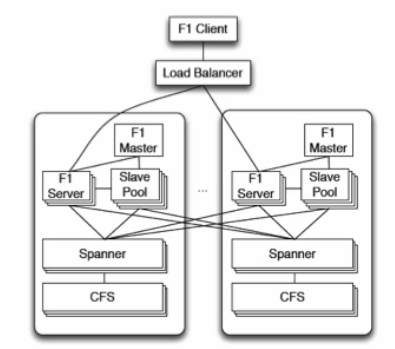
\includegraphics{pics/f1architecture.png}
\end{center}

Here, each the two different containers represent different data centres. Note how the spanner can be accessed by other data centres. Additionally, it uses CFS (colossal file system) rather than GFS, which is not available for use globally yet, so spanner will stay using the local form of it.

F1 master, F1 server and the slave pool work like \texttt{mapreduce}. The servers themselves own no data so easy to change

\subsubsection{Data layout}
Instead of as in a typical RDB, the primary \textit{contains} the foreign keys, so it is easy to know where to go to look for things and save going to and from multiple machines.

\section{The Hadoop Ecosystem}
Originally, there was Hadoop, which is Apache's answer to MapReduce. Of course, Hadoop needed something like GFS, which Apache dubbed HDFS.
BigTable was needed, and this was called HBase. These three projects were known as `The Hadoop Core'.

Writing MR jobs is pretty tricky, so some programmatic abstraction was required. This was called Apache Pig. Additionally, they needed an SQL-like query language, which they called Apache Hive.

\textbf{Mahout} is Apache's scalable machine learning platform, and runs on Hadoop/Spark. It provides tools for using Hadoop to create systems that perform clustering, classification, and collaborative filtering at high sped on large data sets.

\textbf{Giraph} is a graph database system used by Hadoop.

\textbf{YARN} (yet another resource navigator): performs cluster resource management and acts as middleware between HDFS and other applications. Hands out RAM and other resources.

\textbf{HBase/Hoya}: \textit{Hoya} is a tool for running HBase clusters on YARN. HBasse is Hadoops non-relational (noSQL) distributed database (discussed above, v close to BigTable).

\textbf{Kafka}: Distributed streaming platform to store and process streams of records that is written in scala. Uses messaging system for transferring data. Uses zookeeper to share and save states between brokers. In short, you use Apache Kafka as a \textit{distributed} and \textit{robust queue} that can handle \textit{high volume data} and enables you to pass messages from one point to another

\textbf{Storm}: A distributed real time stream processing system, originally by twitter, now an apache project. Much faster than Kafka (I think) Storm allows for creation of even driven processing networks which operate continuously in real-time in comparison to MRs batch-mode style of working and can run on YARN. In short, it is a system that has \textit{distributed real time processing abilities}, meaning you can execute a number of manipulations on \textit{real time data in parallel}

\textbf{Spark}: High performance analytics engine/framework for large scale data-processing that runs on YARN (and other platforms including EC2 and K8s). Uses \textit{in-memory} rather than MRs constant read/writes to hard drive making it very much faster.

\textbf{Flume/Sqoop}: Sqoop transfers data between Hadoop and external datastores. Flume is focused on collecting, aggregating, and moving large log files to external places..

\subsection{Hive}
Hive is best suited to \textit{data warehousing}. It operates on relatively static data where the response time is not critical. It has its own SQL-like query language called HiveQL/HQL, which is much more concise than lower level MR code.

Routes into Hive could either be a CLI, a web interface, or programmatically. Hive has a \textbf{driver} that compiles input, optimises computation and executes subjobs.

\subsection{Pig}
Pig is actually short for Pig Latin, and works on HDFS and NoSQL. Users describe how data is read/processed/stored in parallel. Dataflows could be linear or DAG (directed, acyclic graph). Interestingly, it has no if/for/while. Unlike SQL/HQL, Pig allows users to describe exactly how data will be processed.

\subsection{Cascading}
Similar to Hive and Pig, it is another layer on Hadoop, extending its use. It is still in development. Cascading lets you specify plans for queries. It provides a set of operators and tools for combining them into a DAG (as used in Pig). Each vertex in the DAG is an operator, and data flows from operator to operator. Therefore, it's very similar to Pig, except the graph can be displayed.

Once one job is finished, the next queued job is woken up, and then begins executing.

% ================ WORK DONE 16/09 ===============================
\section{Cloud Databases: NoSQL}
NoSQL is a really good answer to traditional RDBMs since as databases got bigger, people designed bigger single servers, where costs increase nonlinearly. Even when scaled up, they suffer from `inelasticity', in that it's hard to scale them back down again when demands reduced. Instead,  on clusters of cheap commodity servers and don't need ACID. We'll look at different types of NoSQL databases

\subsection{Key-Value DBs}
This is the simplest of NoSQL DB types. There are virtually no constraints (schemaless). A consequence of this is that they are often very fast, and don't require a heavy up-front investment in designing schema and are essentially similar to an associative array that allows any value (no typing restrictions).

Keys must be unique within any one of the KV namespace, which may be the whole DB or one of several buckets within a DB.

Values can be pretty much any digital object.

KV pairs are often mapped to server nodes via a hash function to balance storage or processing load over them. There is no standard for KV datastores; different KVs have differing constraints:
\begin{itemize}
    \item Some offer ACID transactions
    \item Some allow very big objects in values, while others have hard limits
    \item Some constrain data-types of keys to be only string/numbers.
\end{itemize}

Some KV systems have built-in indexing of values:
\begin{itemize}
    \item As KV pairs are added to DB, an index is compiled of unique values
    \item Produces a value->key LUT; index tells you all the keys for a given value.
\end{itemize}

Some KV systems auto-compress.

Schemaless has advantages such as being trivially easy to add things like two key-value pairs on one item, but it doesn't do things like semantic checks, so if you mistype a key, it becomes very difficult to retrieve the value.

\subsubsection{SimpleDB}
Amazon's key-value database.
\begin{itemize}
    \item Items not stored in a table, but in a hierarchical structure
    \begin{itemize}
        \item Domain
        \item Items
        \item Attributes (actual k-v pairs)
    \end{itemize}
    \item Data is all stored as \textbf{text}
    \item Query language is \textit{very basic}
    \item Suffers from eventual consistency.
\end{itemize}

\textbf{DynamoDB} is the updated version of simple DB, although simple DB is still offered. DynamoDB combines document and kv datastores.

\subsubsection{Google App Enging (GAE) Datastore}
Google's key-value database.
\begin{itemize}
    \item Cloud style is scale out, not up, and this is automated
    \item GQL --- Query language
    \item Similar to SimpleDB in structure, but different names:
    \begin{itemize}
        \item Kind
        \item Entities
        \item Properties (with names and values)
    \end{itemize}
    \item Queries into datastore can return entire entities, or just the keys 
    \item Interestingly offers \textit{query pre-indexing}
    \begin{itemize}
        \item During development and testing, queries are recorded, meaning those queries are lightning fast
        \item List of these queries can be edited
        \item Adding and removing entities is a pain, but tradeoff is worthwhile
    \end{itemize}
\end{itemize}

\subsection{Document Databases}
Document DBs manage more complex data structures than KV datastores. They are NOT stores of electronic documents.

Like KVs, DocDBs don't require you to define a common structure for all records in the data store. Unlike KVs, DocDBs allow you to query and filter collections of documents as you would rows in a RDB table.

In NoSQL, a `document' is a structured object: it contains information not only about the data being stored, but also how that data is structured. A document in a DocDB is at root a set of KV pairs, but some of the values can themselves be sets of KV pairs. These documents within documents are called \textit{embedded documents}

Most commonly, documents are described as JSON or XML files.

\subsection{Columnar DBs}
Column-family DBs, or columnar DBs, are used for the really big data. The technical term is VLDB, very large DB. Scaling for previously discussed DBs is possible, but are either hard, or extremely costly. Google's BigTable was the birth of `column family' DBs.

`Column family' comes from the fact that groups of related columns that are frequently used together can be gathered into groups, called families. columns within a family are kept together on disk, to reduce access times.

The data-modeller defines the column \textit{families} prior to implementing the DB, but devs can subsequently add columns to a family.

This means the designer of a DB specifies only a course grained structure. Column families are analogous to keys in KVDBs, with similar constraints wrt uniqueness of names in a namespace

Like DocDBs, ColFam DBs do not require column entries in all rows.

\subsection{Graph DBs}
Some forms of data are most naturally represented in a database as a set of nodes, edges joining nodes to represent relationships between them (many to many relationships that is difficult for RDBMs and SQL).

Specialised graph databases have been developed for efficient storage of such data.

Most graph algorithms are iterative, travers the graph in some way, so MapReduce approach does not map onto graph processing very well.

Neo4J is a newer development that seems to be en route to becoming the de facto standard and outperform Apache's Giraph. 

\section{Queues and Real-time Stream Processing}
We have already talked about message queues, but here is a recap:
\begin{itemize}
    \item Asynchronous
    \item Decoupling
    \item Resilience
    \item Redundancy
    \item Guarantees
    \item Scalable
\end{itemize}

However, message queues provide no transformation or processing.

Apache Kafka was originally used by LinkedIn, before being released as open source. Here are some of the features:
\begin{itemize}
    \item Full independence of the producer and consumer
    \item Persistence
    \item Distributed and replicated
    \item Streams of records stored in categories called topics
    \item Guarantees:
    \begin{itemize}
        \item Messages are appended in the order they are sent
        \item Messages are consumed in the order they are stored
        \item A replication factor $N$, meaning up to $N-1$ server failures are tolerated without losing messages
    \end{itemize}
\end{itemize}

Kafka has a log-based queue, and this is the basic persistence method used. Logs are sharded and replicated, ensuring topics are not limited to one node's capacity. It also uses a pub/sub strategy, but offers extra features, such as record persistence and replication, in a similar manner to many queues.

Kafka is critically dependent on Zookeeper. ZK is a distributed configuration adn synchronisation service, where Kafka stores basic metadata about clusters, consumers, etc.

There are a number of advantages that Kafka has over things like message queues. Kafka consumer groups can function as a queue. It also allows you to broadcast messages like pub-sub, but has the advantage that the Topic structure has both queue and pub/sub properties and can handle scale processing.

\subsection{Real-time stream processing}
Stream processing is the method by which data is processed from a continual stream of raw data, and can be used in things such as the Large Hadron Collider. It is necessary where there is an insane amount of data that needs to be processed \textit{in real time}

We require both high throughput and low latency, along with fault tolerance, since the data needs to be processed as and when it arrives, it doesn't work if there is high latency. RTSP is also `straggler tolerant', where a straggler is an individual task who's execution time is taking much longer than expected.

A stream processor has a framework providing queueing or message passing (push/pull pipelines or pub/sub).

The architecture of RTSP is as follows:
\begin{itemize}
    \item \textbf{Source operator} --- Takes data from a source and turns it into standard message format. This would be where Kafka is.
    \item \textbf{Continuous operator} --- Real time processing and \textit{extract, transform, load} (ETL), into some data analytics. This is where the likes of Apache Spark comes in.
    \item \textbf{Sink operator} --- Data storage
\end{itemize}


When considering RTSP, data needs to be considered:
\begin{itemize}
    \item Data sources: How is the data stored? (binary/string)
    \item Size: How big is the data?
    \item Order
\end{itemize}

It is required that messages are delivered \textit{exactly once} and messages are guaranteed to be delivered in the order they were sent. (always once and exactly once)

We can use Kafka for stream processing, too. There are three approaches to extend Kafka to handle this:
\begin{itemize}
    \item Do it yourself
    \begin{itemize}
        \item Looks simple
        \item But is actually hard
    \end{itemize}
    \item Fully fledged stream processing system
    \begin{itemize}
        \item Apache Storm, Spark, Flink, Samza
    \end{itemize}
    \item Lightweight stream-processing library
    \begin{itemize}
        \item Kafka streams included in Kafka for ages, which is powerful and easy to use.
    \end{itemize}
\end{itemize}

\section{Spark}
Complex jobs, interactive queries and online processing all need efficient primitives for data sharing, but in MapReduce, the only way to share data across jobs is stable storage (like the file system).

MapReduce would require a lot of I/O operations, and these calls could take up to 90\% of the processing time. An alternative to this is \textit{in-memory data sharing}. The basic idea is that we just write, well, in memory, rather than return to the disk every time. It can be between 10 or 100 times faster.

Spark and other \textbf{resilient distributed databases (RDDs)} is the technology that allows this.

\begin{tcolorbox} [space to upper,
collower=white,
title={RDD},
nobeforeafter,
halign lower=flush right, ]
An Rdd is:
\begin{itemize}
    \item An immutable, partitioned, logical collection of records that can be stored in memory across the cluster
    \item May be partitioned by a key in each record
    \begin{itemize}
        \item A key that partitions in a smart way improves performance
    \end{itemize}
    \item May not be \textit{materialized} until needed
    \item May be \textit{cached} in memory if repeated use is anticipated (can also tell the system to cache data)
\end{itemize}
\end{tcolorbox}

RDDs are created and manipulated through applying bulk transformations on disk or in memory (map, filter, join). Outputs to the driver node are generated by applying actions in parallel to RDDs (reduce, collect, count). RDDs are \textit{lazy}; they don't materialize data until absolutely necessary.

Using an example of Log mining, we can load error messages from a log into memory and then interactively search for various patterns (in scala):
\begin{lstlisting}
lines = spark.textFile("hdfs://...") 'base RDD
errors = lines.filter(_.startsWith("ERROR")) 'transformed RDD
messages = errors.map(_.split("\t")(2)) 'also transformed RDD
messages.cache() 'expected to use it again, so cached RDD

messages.filter(_.contains("foo")).count
messages.filter(_.contains("bar)).count
\end{lstlisting}

we have to care about fault tolerance in RDDs quite a lot, so here's how it is done:
\begin{itemize}
    \item Fault recovery without costly replication:
    \begin{itemize}
        \item Rather than just checkpointing data
        \item Just remember the series of transformations that built an RDD and use this series to re-compute the lost data if required.
    \end{itemize}
    \item  
\end{itemize}
% ===================================================================

%======================work on 19-09===================================
\subsection{Example: Logistic Regression}
If we have a number of data points (some negative, some positive), can we use a point $x$ to predict its $y$? And can we find the best way to linearly separate two sets of D-dimensional points? We can use $w$, a vector of $D$ weights:

If $(1+e*{-w\cdot x})^{-1}>0.5$, we guess positive, else negative. We can iteratively improve an initially random $w$ using gradient descent:
\begin{align*}
w_{new} \rightarrow w - a\bigg( \frac{1}{1+e^{y\cdot wx}} -1\bigg)
\end{align*}

Where $a$ is the learning rate. Each iteration, we consider a new point.

Here's a piece of code we can feed into Spark:
\begin{lstlisting}[language=Python]
def parsePoint(line):
    values = [float(x) for x in line.split(' ')]
    return (values[0], values[1:D])

points = spark.textFile(...).map(parsePoint).cache()

w = numpy.random.ranf(size = D)

for i in range(N):
    gradient = points.map(
            lambda.p: (1/(1+exp(-p.y*(w.dot(p.x))))-1)*p.y*p.x
    ).reduce(lambda a, b:a + b)
    w -= alpha*gradient #learning rate
\end{lstlisting}

When this is implemented with Hadoop, the number of iterations raises quite dramatically, while with Spark, it is much slower (running-time wise). This is because we are able to utilise the in-memory storage effectively. Spark has a slightly higher overhead at the beginning as it is building the RDDs and setting up images, so the first iteration will be marginally slower than Hadoop for the first few iterations, but once this is set up the incremental running time is dramatically lower.

\subsection{Spillover}
If memory objects are too large, they are written to disk and handled in a standard manner. No slower than MapReduce. Logistic regression performance varies depending on how much of the memory of the data is cached in memory vs. spilling onto disk. Performance degrades \textit{gracefully} (meaning gradual decline, not like a cliff).
%+=====================================================================

%============= WORK DONE 24/12 =================
\section{Sustainability and Cloud Computing}
\subsection{Theoretical Frameworks}
A simple tool to help reasoning between economic and environmental impact is the $I = P \times A \times T$ and decoupling. Simply, this is Impact = Population $\times$ Affluence $\times$ Technology.
\begin{itemize}
    \item The \textit{population} refers to the population of an area, such as the world.
    \item \textit{Affluence} represents the average consumption of each person in the population. A common measure for this is GDP per capita.
    \item \textit{Technology} is how resource intensive the production of affluence is; how much environmental impact is involved in creating, transporting and disposing of the goods, services, adn amenities used.
\end{itemize}

The \textbf{rebound effect} is the reduction in expected gains from new technologies that increase the \textit{efficiency} of resource use because of behavioural or other systemic responses. These responses diminish the beneficial effects of the new technology or other measures taken.

The \textbf{3-level Framework} of environmental impact of ICT was introduced as a measure of the impact of computer systems on the environment. ICT can be either part of the problem, or part of the solution, depending on the actual problem.
\begin{enumerate}
    \item \textbf{Direct effects}
    \begin{itemize}
        \item Life cycle phases
        \begin{itemize}
            \item Raw material extraction, manufacturing and assembly, etc.
            \item Use: Electricity, Diesel, water
            \item Disposal: Land Fill, Incineration, Recovery of material (recycle)
        \end{itemize}
        \item Assessed with the LCA (Life Cycle Assessment) to quantify the impact (these are all negative).
    \end{itemize}
    \item \textbf{Enabling effects}
    \begin{itemize}
        \item Application of ICT
        \item Negative
        \begin{itemize}
            \item Induction --- Stimulation of consumption of another resource (printer causing increased paper consumption)
            \item Obsolescence --- Putting something out of date (iPhones for example)
        \end{itemize}
        \item Part of the solution
        \begin{itemize}
            \item Substitution --- Use of ICT for replacement of another resource (Kindle replacing physical books)
            \item Optimisation --- Use of ICT to reduce the amount of resources required for a process through greater efficiency.
        \end{itemize}
    \end{itemize}
    \item \textbf{Systemic effects}
    \begin{itemize}
        \item Negative
        \begin{itemize}
            \item Rebound effects
            \item Emerging risks
        \end{itemize}
        \item Positive
        \begin{itemize}
            \item Transition towards sustainable patterns of production and consumption
        \end{itemize}
    \end{itemize}
\end{enumerate}

The effects on the third level are complicated and often shied away from. It is important to take heed of them, however. They can be more significant than the micro-economic level effects observed in levels 1 and 2.

\subsection{Direct Footprint}
Here are some ideas to keep ICT green:
\begin{itemize}
    \item Design for environmental sustainability
    \item Energy-efficient computing
    \item Power management
    \item Data center design, layout and location
    \item Server virtualisation
    \item Responsible disposal and recycling
    \item Regulatory compliance
    \item Environment-related risk mitigation
    \item Use of renewable energy sources
    \item Eco-labeling of IT products
\end{itemize}

\subsection{Datacentre Sustainability}
Datacentres themselves have an impact on the environment and it is important to reduce the footprint of them. The impact they have includes:
\begin{itemize}
    \item Electricity consumption
    \item Devices: servers and networking
    \item Water for cooling
    \item Resources included in construction of datacentres
    \item Diesel for generators (backup power)
\end{itemize}

Globally, it is estimated that data centres use around 200TWh globally. This has stabilised somewhat since 2014 due to the move to cloud, as there were some fears surrounding data centres at this time, however, they did not materialise.

\subsection{Reporting Tools}
Carbon reporting is a method for reporting the amount of carbon used. This reporting has experienced a lot of innovation recently, with Microsoft Azure, and Google's dashboard for their carbon usage for example. It is now mandatory for organisations to be transparent with the amount of carbon they produce. Google's tools are very advanced, such as using location-based and rack-level monitoring.

For efficient cloud computing, it is important to:
\begin{itemize}
    \item Reduce the PUE (power usage efficiency)
    \begin{itemize}
        \item For example, relocate to colder areas to save on cooling
    \end{itemize}
    \item Inter-datacentre or temporal load balancing
    \item Recycling and reusing their kit.
    \begin{itemize}
        \item Servers have a lifespan of 5 years, but their components might still be useful
    \end{itemize}
    \item Energy efficient devices
    \begin{itemize}
        \item More costly, but could save overall
    \end{itemize}
\end{itemize}

For us, the user, here are some things we can do:
\begin{itemize}
    \item Use a green hoster
    \item Efficient caching is \textbf{the most consistent} way to reduce emissions
    \item Use CDNs
    \item Favour serverless (FaaS)
    \item Auto-scaling
    \item Avoid top-of-the-hour for scheduled jobs and add jitter
    \item Remove unneeded data
    \item Use spot instances for workloads that require both batch processing, reduces unused capacity
\end{itemize}

\subsection{Cloud Application Assessments}
Streaming uses creates quite a lot of carbon, and there is carbon reporting for digital services available.

\section{Legal Aspects}
\subsection{Open Source}
Open source means that code is publicly accessible. Anyone can read it or contribute to it. Not open source software has a legal relationship and is protected as a work of literature.

When we normally think of open source, we are thinking of `free' open source software.

How does it work?
\begin{enumerate}
\item Quality
\begin{itemize}
    \item Because the code is available for everyone to view, it is likely that all bugs will be captured; even the really obscure one. If you find a bug, you can just pinpoint it and fix it yourself.
    \item Linus' Law: Given enough eyeballs, all bugs are shallow
\end{itemize}
\item Network effects
\begin{itemize}
    \item Tensorflow
\end{itemize}
\item Brand building
\begin{itemize}
    \item VCS
    \item Distributed
    \item Pull requests
\end{itemize}
\end{enumerate}

\subsection{Licenses}
A license is:
\begin{itemize}
    \item A legal instrument governing the use or redistribution of software
    \item They are not patents (protecting an invention)
    \item A license protects a specific piece of software
\end{itemize}

You need a license because without a license, no one is able to reproduce, distribute, or create derivative works. Everybody who contributes to your project also becomes an exclusive copyright holder and it becomes very messy. To use the code, you must contact the author directly and ask permission.

You need to choose a license (two types):
\begin{itemize}
    \item Permissive: allow users to do what they want
    \begin{itemize}
        \item MIT --- Do anything, but don't sue me lol
        \item Apache --- like MIT, but with more boilerplate (explicit patent license, good for business use)
    \end{itemize}
    \item  Copyleft (`viral'): 
    \begin{itemize}
        \item GPL v2/3 (gnu public license) --- if you link to a GPL library/piece of software, you need to redistribute your own software under GPL also (your software needs to be open source)
    \end{itemize}
\end{itemize}

\subsection{Data Protection}
UK privacy and electronic communications (PECR) has a `cookie law'. This is designed for users to consent when someone stores a piece of information on your local machine. It's the whole allow decline shit we have to deal with these days. Information should enable users to understand the use of cookies and must be accessible after consent. Revoking consent also needs to be accessible.

\subsection{GDPR}
GDPR is the law to govern privacy of all EU citizens around the world and give them control over their personal data. Fines for not following this is €20 million or 2\% up to 4\% of the total worldwide annual turnover, whichever is greater.

\textit{Personal data} means any information relating to an identified or identifiable natural person ('data subject'). An identifiable natural person is one who can be identified, directly or indirectly, in particular by reference to an identifier such as a name, identification number, location data, an online identifier or to get one or more factors specific to the physical, physiological genetic, mental, economic, cultural, or social identity of that natural person.

Common categories include:
\begin{itemize}
    \item Biographical information
    \begin{itemize}
        \item Dates of birth
        \item Social security numbers
        \item Phone numbers
        \item Email addresses
    \end{itemize}
    \item Appearance and behaviour
    \begin{itemize}
        \item Eye colour, weight
    \end{itemize}
    \item Workplace data and information about education
    \begin{itemize}
        \item Salary
        \item Tax information
        \item Student numbers
    \end{itemize}
    \item Private and subjective data
    \begin{itemize}
        \item Religion
        \item Political opinions
        \item Geo-tracking data
    \end{itemize}
    \item Health, sickness and genetics
    \begin{itemize}
        \item Medical history
        \item Genetic data
        \item Information about sick leave
    \end{itemize}
\end{itemize}

The rules surrounding this data are that:
\begin{itemize}
    \item No personal data may be processed without unambiguous and individualised consent from the data subject.
    \item The processing of personal data should be limited to what is necessary for the purposes for which they are processed
    \item Controllers of personal data need appropriate technical and organisational measures (such as encryption, pseudo or full anonymisation)
    \item Right to revoke this consent
    \item Declare any data collection and purpose for data processing, and state how long the data is retained
\end{itemize}

This mainly applies to EU countries, but also restricts the transfer of data outside the EU. Some countries are covered by the adequacy decision in 2019 (Andorra, Argentina, Guernsey, Isle of Man, Israel, Jersey, NZ, Switzerland and Uruguay).

In the USA, it works slightly different (and this is only for companies under the EU-US privacy shield framework):
\begin{itemize}
    \item Government audited
    \item Checklist of companies
    \item Certain type of data
\end{itemize}

SCCs (standard contractual clauses):
\begin{itemize}
    \item Legal instrument between sender and receiver to guarantee data protection
    \item ICO tool
\end{itemize}
%===============================================

\section{Cloud Security}
Cloud security has been a major concern and research issue from the earliest days of serious use of cloud computing. The \textbf{cloud security alliance} (CSA) is a non-profit collaboration between an impressive number of major players.

The CSA in 2013 identified nine notorious threats:
\begin{enumerate}
\item Data breaches
\item Data loss
\item Account hijacking
\item Insecure APIs
\item Denial of Service
\item Malicious Insiders
\item Abuse of Cloud Services
\item Insufficient Due Dilligence
\item Shared Technology Issues
\end{enumerate}

And then updated this in 2016 to the `treacherous twelve':
\begin{enumerate}
\item Data breaches (\#1)
\item {\color{red} Identity/credential/access management}
\item Insecure APIs (\#4)
\item {\color{red}System Vulnerabilities}
\item Account hijacking (\#3)
\item Malicious Insiders (\#6)
\item {\color{red}Advanced Persistent Threats}
\item Data loss (\#2)
\item Insufficient Due Dilligence (\#8)
\item Abuse (and nefarious use) of Cloud Services (\#7)
\item Denial of Service (\#5)
\item Shared Technology Issues (\#9)
\end{enumerate}

And most recently, the `egregious eleven' in 2019, which is missing numbers 4,7,8,9,11, and 12 from the treacherous twelve:

\begin{enumerate}
\item Data breaches
\begin{itemize}
    \item When an organisations sensitive data falls into the hands of a competitor
    \item For example, corporate IT rules being circumvented
\end{itemize}
\item {\color{red}Misconfiguration and inadequate change control}
\begin{itemize}
    \item Misconfiguration occurs when assets are setup incorrectly leaving them vulnerable to malicious activity
    \item Common examples include unsecured data storage elements, lax permissions, etc.
    \item Misconfiguration of cloud resources is a leading cause of data breaches.
\end{itemize}
\item {\color{red}Lack of cloud security architecture and strategy}
\begin{itemize}
    \item Main example given is Accenture's massive release of internal passwords and access keys of its enterprise cloud offering, via four unsecured AWS S3 buckets. Basically released the master key by accident.
\end{itemize}
\item Insufficient identity/credential/access management
\begin{itemize}
    \item Data breaches and enabling of attacks can occur because of a lack of scalable identity access management systems, failure to use multi-factor authentication, weak password use, and a lack of ongoing automated rotation of keys, passwords and certificates.
\end{itemize}
\item Account hijacking
\begin{itemize}
    \item Phishing, fraud, software exploits, etc.
\end{itemize}
\item Insider threat
\begin{itemize}
    \item A malicious insider, such as sysadmin, in an improperly designed cloud scenario can have access to potentially sensitive information.
\end{itemize}
\item Insecure interfaces
\begin{itemize}
    \item Composing services from large numbers of orchestrated component services raises the risk that one or more of the component APIs could be weak and/or compromised. Spreading out keys or tokens over the components magnifies this risk.
\end{itemize}
\item {\color{red}Weak control plane}
\begin{itemize}
    \item The management plane of a cloud service is critical and needs to be adequately protected by identity and access controls. 2FA should be part of the standard suite of controls provided to a cloud customer by the cloud service provider, but many only make this available to their customers as a premium service.
\end{itemize}
\item {\color{red}Metastructure and applistructure failures}
\begin{itemize}
    \item \textbf{Metastructure} is metadata that describes the cloud architecture
    \item \textbf{Applistructure} is technology infrastructure and business applications
    \item Both of these are critical components of a cloud service that, if they fail at CSP level, can severely impact all consumers.
\end{itemize}
\item {\color{red}Limited cloud usage visibility}
\begin{itemize}
    \item This occurs when an organisation does not possess the ability to visualise and analyse whether the cloud service use within the org is safe or malicious.
    \item There are two key challenges: unsanctioned app use (unknown apps being used) and sanctioned app misuse (using known apps in bad ways).
\end{itemize}
\item Abuse (and nefarious use) of cloud services
\begin{itemize}
    \item It might take an attacker years to crack an encryption key using their own hardware, but using an array of cloud servers, it can be done in minutes. Also, DDoS becomes quite easy using these servers.
\end{itemize}

\end{enumerate}

It was noted after analysis that there was a drop in ranking of traditional cloud security issues under the responsibility of the service providers such as DoS, etc. They were rated so low they were not included in the rankings. Newer, more highly rated items imply a higher maturation of the consumer's understanding of the cloud, where the issues are really specific to the cloud and indicate a landscape where consumers are actively considering cloud migration.
\end{document}